\section{Exercise 7.13 Human voice analysis}
\subsection{MATLAB Implementation}
\lstinputlisting[caption={MATLAB script \texttt{dft\_voice.m}}, label={lst:dft_voice}]{Code/dft_voice.m}

\subsection{Results}

\begin{figure}[H]
    \centering
    
\includegraphics[width=1\linewidth]{Figures/a_low_spectrum.png}
    \caption{A low power spectrum}
    \label{fig:placeholder}
\end{figure}

\begin{figure}[H]
    \centering
    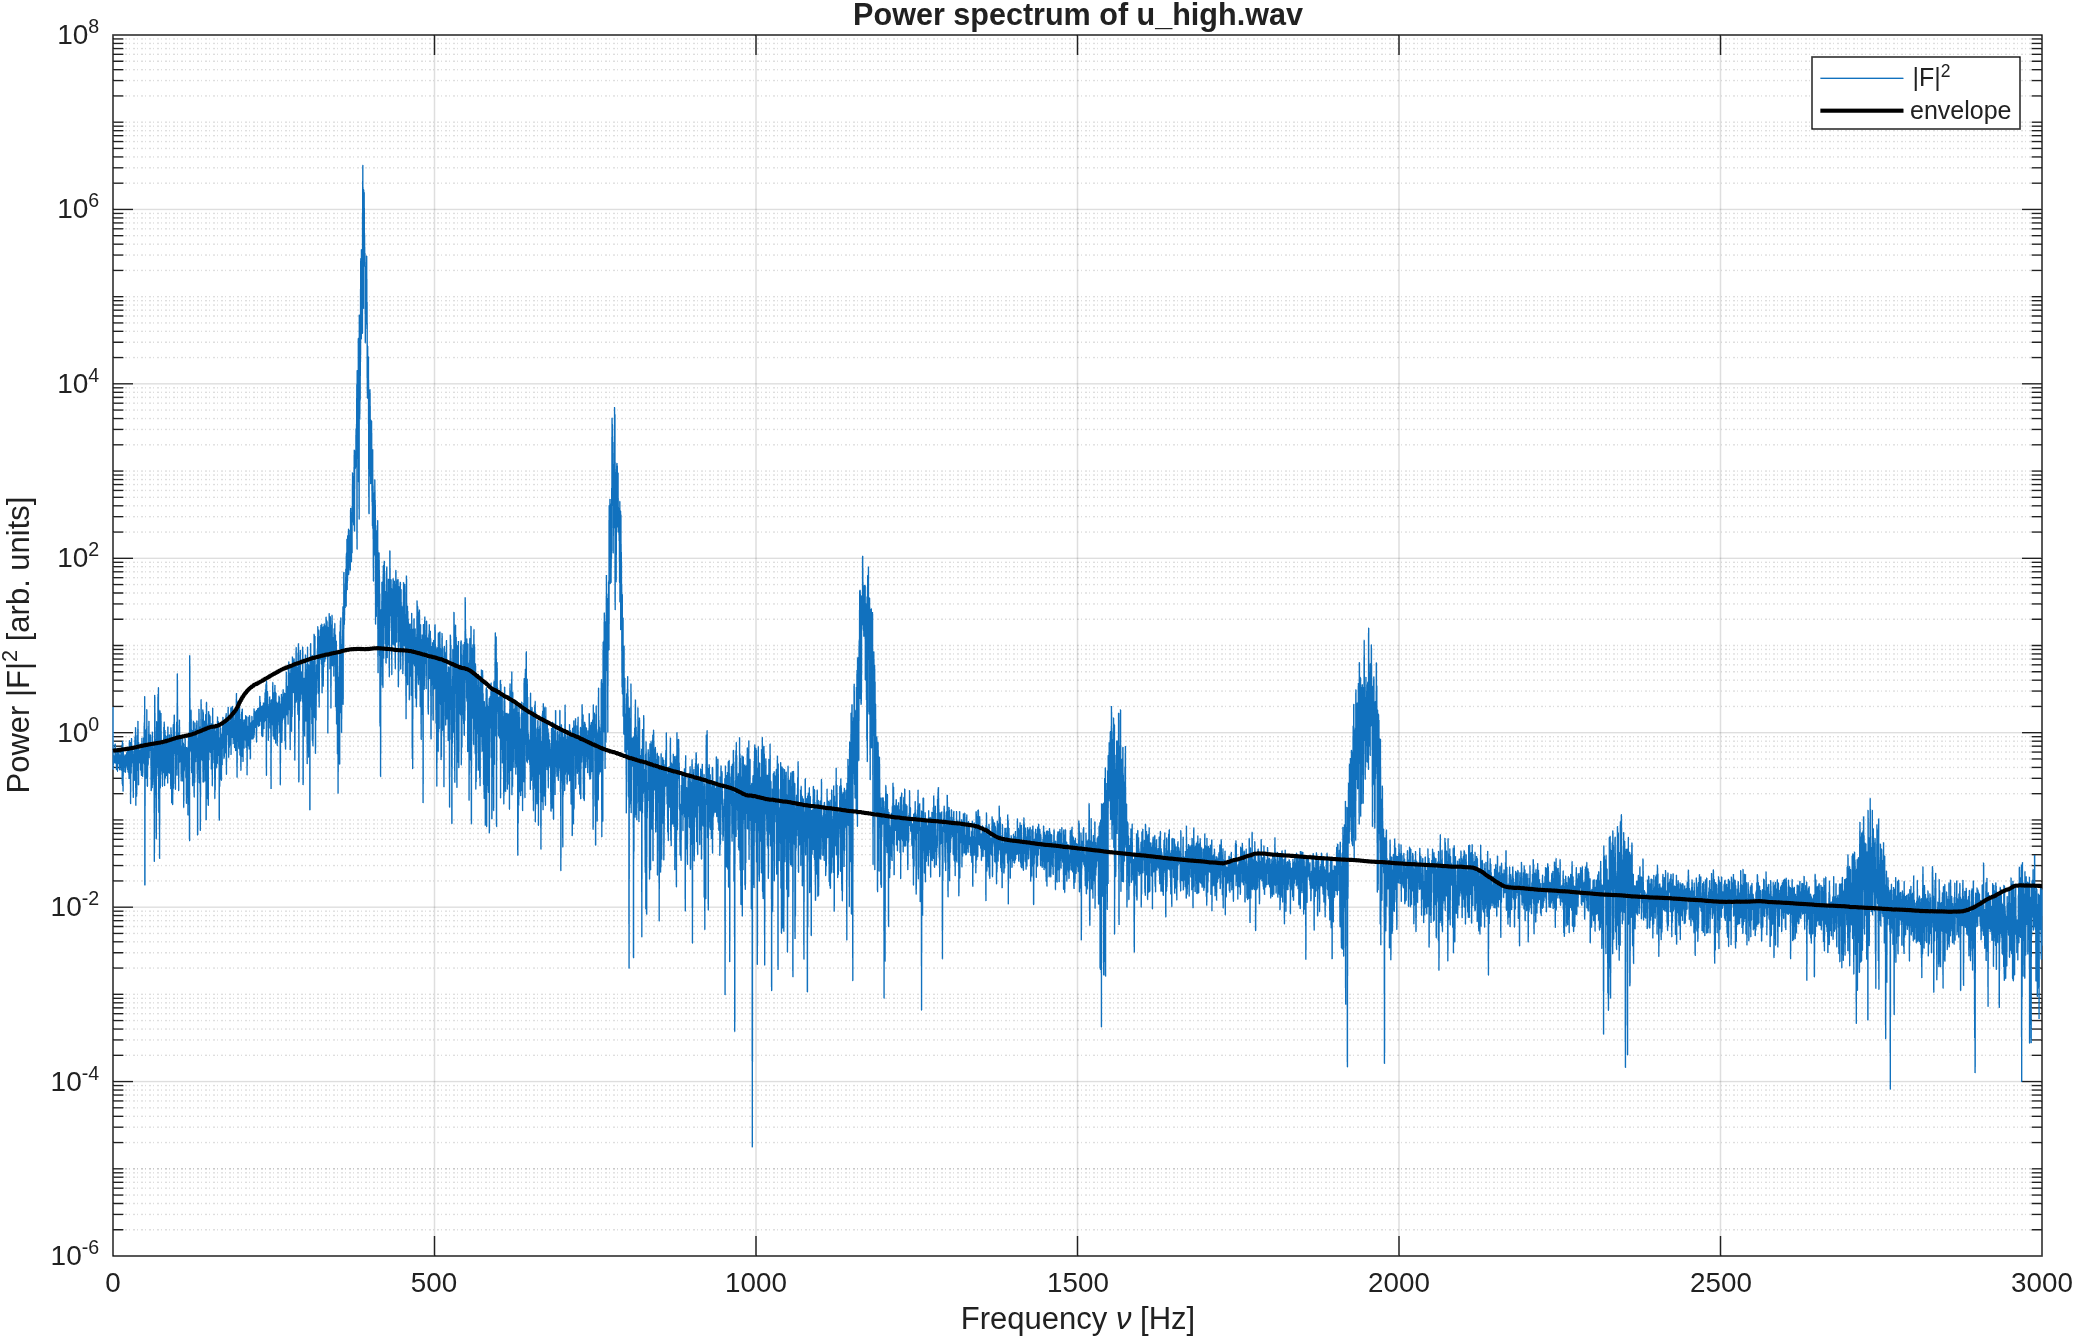
\includegraphics[width=1\linewidth]{Figures/u_high_spectrum.png}
    \caption{U high power spectrum}
    \label{fig:placeholder}
\end{figure}

\begin{figure}[H]
    \centering
    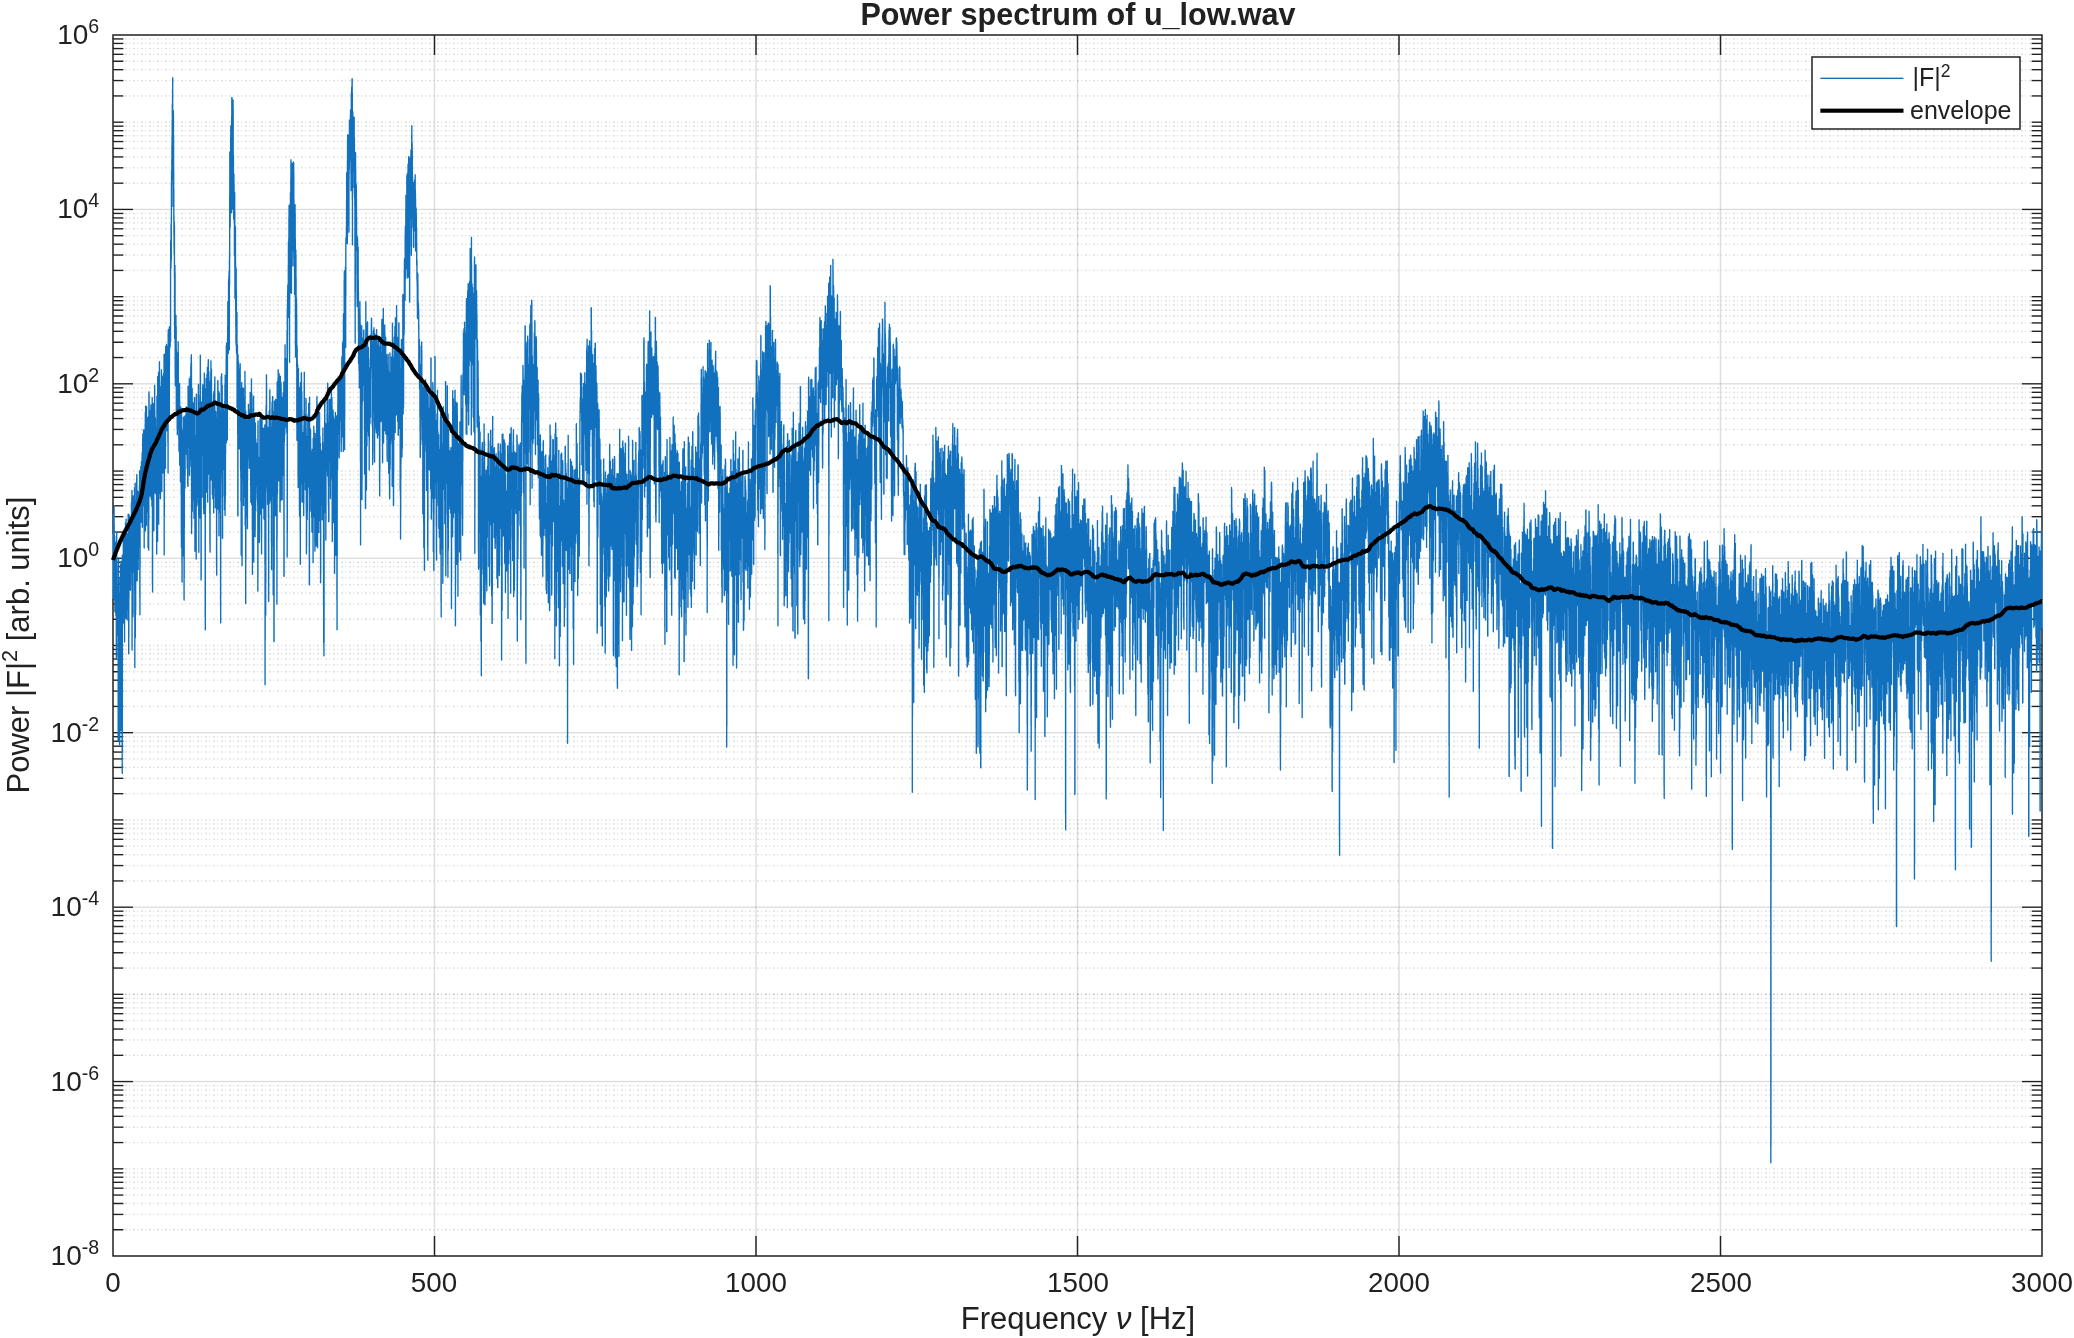
\includegraphics[width=1\linewidth]{Figures/u_low_spectrum.png}
    \caption{U low power spectrum}
    \label{fig:placeholder}
\end{figure}

\begin{table}[H]
    \centering
    \caption{Base frequencies for all voice recordings}
    \label{tab:placeholder}
    \renewcommand{\arraystretch}{1.2}
    \begin{tabular}{lc}
        \toprule
        A low   & 92.8 Hz \\
        U low   & 92.8 Hz \\
        U high  & 388.5 Hz \\
        \bottomrule
    \end{tabular}
\end{table}


\begin{table}[H]
    \centering
    \renewcommand{\arraystretch}{1.2}
    \small
    \begin{minipage}[t]{0.44\textwidth}
        \centering
        \caption{Measured formant frequencies (Hz), read from the power spectra}
        \label{tab:formants}
        \begin{tabular}{lcc}
            \toprule
            File   & $F_1$ & $F_2$     \\
            \midrule
            A low  & 750   & 1175      \\
            U low  & 400   & 1125      \\
            U high & 400   & not clear \\
            \bottomrule
        \end{tabular}
    \end{minipage}\hfill
    \begin{minipage}[t]{0.54\textwidth}
        \centering
        \caption{Predicted formant frequencies (Hz), read from figure D.8}
        \label{tab:formants_pred}
        \begin{tabular}{lcccc}
            \toprule
                        & \multicolumn{2}{c}{Men} & \multicolumn{2}{c}{Women} \\
            \cmidrule(lr){2-3} \cmidrule(lr){4-5}
            Vowel       & $F_1$ & $F_2$ & $F_1$ & $F_2$ \\
            \midrule
            a           & 770   & 1290  & 980   & 1430  \\
            \textipa{A} & 670   & 1050  & 760   & 1100  \\
            u           & 400   & 830   & 330   & 840   \\
            \bottomrule
        \end{tabular}
    \end{minipage}
\end{table}

\pagebreak 
\subsection{Result analysis}
The base frequency is $\nu_0 = 92.8$~Hz for both u\_low and a\_low, and $\nu_0 = 388.5$~Hz for u\_high. In the spectra of u\_low and a\_low, the higher harmonics are clearly visible as peaks at integer multiples of $\nu_0$, and the envelope shows several formants. For u\_high the harmonics are also visible, but they lie so far apart that only the first formant can be distinguished in the envelope.

The measured formant frequencies are listed in table~\ref{tab:formants} and the predicted values in table~\ref{tab:formants_pred}. For a\_low, both the first and the second formant agree reasonably well with the predicted values for /a/. For u\_low, the first formant matches the prediction, but the second formant is about 300~Hz higher than expected. This could be because the vowel was pronounced with less lip rounding, or with the tongue further forward, than by the average speaker, since both raise the second formant. For u\_high, the first formant agrees with the predicted value, but the second formant could not be distinguished, so it cannot be compared.

For u\_low and u\_high, the first formant is located at the same frequency, about 400~Hz. The higher formants are hard to compare, because they are not visible in the envelope of u\_high. The harmonics lie at integer multiples of $\nu_0$, so for u\_high they are 388.5~Hz apart instead of 92.8~Hz: below 3~kHz there are only about 7 harmonics, against about 32 for u\_low, which are too few points to trace the shape of the envelope. The formant of u\_low near 2050~Hz is only hinted at in u\_high by the harmonic near 1940~Hz, which is stronger than the one before it near 1550~Hz. The base frequencies differ by a factor of about 4.2. This is what we expect: the base frequency is set by the vibration of the vocal cords, which vibrate faster for the higher note, while the formants are the resonance frequencies of the cavity formed by the throat and mouth, which depend only on its shape. Both recordings are the same vowel, so the cavity has the same shape and the formants stay in place. This agrees with appendix D: the lower the base note, the closer together the overtones lie and the better the formants are defined.

For a\_low and u\_low, the formants are located at different frequencies: the first formant moves from about 400~Hz to 750~Hz, the second from about 1125~Hz to 1175~Hz, and a higher formant from about 2050~Hz to 2550~Hz, so the first formant changes the most. The base frequency, on the other hand, is the same for both ($\nu_0 = 92.8$~Hz), which can also be seen directly in the spectra as the same spacing between neighbouring harmonics. This is what we expect: both vowels were produced at the same pitch, so the vocal cords vibrate at the same rate, while changing the vowel from u to a changes the shape of the cavity (the mouth opens and the tongue moves), and with it its resonance frequencies. According to appendix D, the first two formants $F_1$ and $F_2$ completely determine which vowel is produced.
